\chapter{Discussion}

In this chapter the technical results of the project are analysed. First, the design verification is performed, showing the simulation and the experimental results. Then, the main impediments found through the project and implementation's limitations are explained. Finally, suggestions for future work are presented.

\section{Validation of experimental results}

\todo{this title i think should be verification the PMBOK guide, a standard adopted by IEEE, defines them as follows in its 4th edition5: ---Validation. The assurance that a product, service, or system meets the needs of the customer and other identified stakeholders. It often involves acceptance and suitability with external customers. Contrast with verification. ---Verification. The evaluation of whether or not a product, service, or system complies with a regulation, requirement, specification, or imposed condition. It is often an internal process. Contrast with validation.}


In this section the experimental results from the open-loop and MPPT test in section \ref{systemtest} are compared with the simulation results from section \ref{sec:componentsizing} and \ref{MPPTSimulation}.
\subsection{Open-loop simulation}

The main losses are the dissipation from the component in heat. Also the load is a power resistor and it changes the resistance if it is in operation. So we have not a constant load at the output as in the simulation. Another reason is the dead-time of the MOSFET and therefore the duty cycle is not exactly the same value as in the simulation. 

The table \ref{tab:ripple} compares the values of the ripples from the experiments with the values from the requirements in section \ref{sec:componentsizing} and the simulation results in appendix \ref{app:OL_ripple}. So in all three cases the measured ripples from the experiment are higher/lower than the values from the requirement. Here the reason.

\begin{table}[H]
	\centering
	\begin{tabular}{|>{\centering}p{3.5cm}|p{3cm}|p{3cm}|p{3cm}|}
		\hline
		\rowcolor{lightgray} \textbf{} & \textbf{Requirement} & \textbf{Simulation}  & \textbf{Experiment}   \tabularnewline \hline
		$\Delta V_{in}$ & 0.1\% & - & - \tabularnewline \hline
		$\Delta I_{L}$ & 10\% & 10\% & 9.86\% \tabularnewline \hline
		$\Delta V_{out}$  & 0.5\% & 0.5\% & 0.055\% \tabularnewline \hline
	\end{tabular}
	\caption{Voltage and current ripple.}
	\label{tab:ripple}
\end{table}

\todo{The output ripple was tested for buck mode instead of boost mode so mention here why. Stef}

\subsection{Maximum Power Point Tracking}

The proposed Perturb and Observe algorithm was simulated and also tested in the PV lab to show its real performance. The simulation was implemented in PLECS beccause this software allows to program easily the C-code for the MPPT algorithm. The results obtained showed MPPT's efficiencies higher than 99\% for the different levels of irradiance and temperature. As mention in previous chapters, the MPPT algorithm was designed with the objective of increasing the power generated by the PV panel. This was achieved in simulations together with fast MPP tracking and low oscillations around the MPP. 

Once the MPPT algorithm was working as expected, it was tested in the PV lab using the RT Box as the MPPT controller \cite{RTbox}. The RT Box received as analog inputs the voltage and current measured at the output of the PV simulator. The digital outputs of the RT Box were the PWM signals for switching the MOSFETs. The experimental setup is shown in figure \ref{testsetup}.

Table \ref{tab:comparisonMPPT} shows the simulated results together with the experimental results The experimental results obtained under STC show that the MPPT's efficiency is higher than 97\%. Therefore, the performance of the proposed P\&O algorithm is in the rate of the most common MPPT algorithm which varies between 96\% and 99\% \cite{MPPTResearch}. For the case of the conventional P\&O algorithm, the MPPT's efficiency is around 96\% \cite{MPPTResearch}. Hence, the modifications applied to the conventional P\&O algorithm allowed to improve the MPPT's performance. 

\begin{table}[H]
	\centering
	\begin{tabular}{|>{\centering}p{2.3cm}|p{2.3cm}|p{2.3cm}|p{2.3cm}|p{2.3cm}|}
		\hline
		 \rowcolor{lightgray} & \multicolumn{2}{|c|}{ \textbf{Buck Mode}} & \multicolumn{2}{|c|}{ \textbf{Boost Mode}} \tabularnewline \hline
		\rowcolor{lightgray} \textbf{} & \textbf{Simulation}  & \textbf{Experiment} & \textbf{Simulation}  & \textbf{Experiment}  \tabularnewline \hline
		$\eta_{MPPT}$ & 99.96 \% & 97.72 \% & 99.82 \% & 97.32 \% \tabularnewline \hline
		$t_{MPPT}$ & 2 s & 10 s & 4 s & 21 s \tabularnewline \hline
		$D$  & 0.8155 & 0.7594 & 0.5971 & 0.5823 \tabularnewline \hline
	\end{tabular}
	\caption{Simulated and experimental results for the P\&O MPPT algorithm under STC.}
	\label{tab:comparisonMPPT}
\end{table}

Comparing the experimental results with the simulated ones, from table \ref{tab:comparisonMPPT}, it is seen that the time the MPPT takes to reach the MPP is five times higher than in simulation \todo{IS IT FAST? ASK THE SUPERVISORS! Stef}. For the duty cycles, the ideal values under STC for buck and boost modes are 0.5900 and 0.8130, respectively. Comparing these values with the obtained results, it is considered accurate enough to validate the P\&O MPPT algorithm.   

\section{Problems and limitations}
3-Explain main problems and limitations and how are handled. Be succinct, be frank but no apologetic. Explain implications of limitations.
\subsection{Layout improvement procedure and issues, title to be improved}
opto <--x-->driver voltage levels?

inductor saturation and so

pcb hot points

...
\subsection{output cap?}
\subsection{MPPT drifting and improvement and limitations of final control algorithm}
The development of an embedded control system requires the proper working of an algorithm. During the development process, the engineer might find that the code doesn't behave as intended. A common way of supporting the debugging process consists on the use of breakpoints, where the code is stopped and the variables' value might be read. However, as this feature is not supported by the used platform, and in the case of controlling physical systems its use would be limited to simulation, alternative techniques had to be used. The adopted approach consisted on outputting the FSMs state and relevant values for the current state at every code execution loop. The 'Timestamp' field is specially important during simulation in order to track specific events at determined times. See figure \ref{console_output}.

\begin{figure}[htbp]
	\begin{center}
		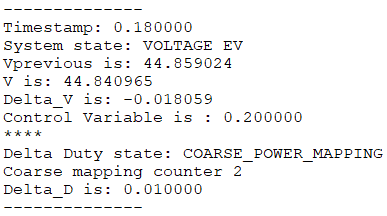
\includegraphics[width=0.5\textwidth]{../Pictures/P1/Discussion/console_output.png}
		\caption{Console output.}
		\label{console_output}
	\end{center}	
\end{figure}

In initial implementations of the control algorithm, the voltage evaluation was performed in the state next to the duty cycle change. After this change, the system experiences a transient stage where the input voltage and inductor current evolve into the new steady state value. If these variables are read during the transient, the control might infer that the PV panel is in a location of the P-V curve different than where it actually is. The MPPT becomes noisier under this scenario. In order to address this issue, an additional waiting state was added to the FSM governing the system. Another solution to the issue would be to decrease the MPPT algorithm periodicity. However this solution would lead to a decrease in system's responsiveness. This drawback might be bearable by implementing a voltage controller aside from the MPPT.  

The noise in measured signals highly influenced the algorithm performance. This noise was addressed by software low pass filtering. The filter caused a dramatic improvement in signal acquisition and system response, further details are explained in the next section.

In order to develop a completely reliable algorithm further testing must be performed. These testing activities require more advanced debugging information than the console output previously shown. RT-box allows SPI communication but the testing activities would still be limited to black-box techniques. In order to reach white-box testing, the implementation would require a microcontroller instead of the RT-box. In that case, the variables' value might be directly accessed with a debugger. Also in the case of black box testing the signals are sent with a known and fixed latency in a microcontroller, which is not the case when using PLECS's console.

The implemented algorithm has more advanced functions than the simplest implementation found in introductory application notes from manufacturers, like \cite{AN1521_MC}. Among the advanced functions are tunable threshold parameters, waiting for the PV to reach open circuit voltage or variable perturb step, among others. However, this additional features add difficulty to testing activities and code comprehension. Under the development of a commercial product, it might be desirable to limit the features in order to decrease test and validation activities' cost. The decrease of the perturb variable itself consists of a FSM with 5 states with a weak coupling with the main FSM. The appropriate testing of the code requires software design and testing knowledge.

The proposed implementation has some variables which might be further optimized, like the initial value of the perturb step value, or the threshold to decrease the perturb step value. 


\subsection{Software filter}
Although the voltage and current measurement is filtered, the signal read by the control system was noisy. This noise affected the MPPT algorithm disturbing its ability to reach the MPP. Such noise might have different sources within a lab with such a big amount of hardware equipment. There are many techniques in order to address noise issues, the used technique consists on the use of digital filtering (LPF). This digital filter is a  simple code that performs the filtering at a given frequency. Being a first order filter, it was simple and fast to implement. The result can be seen in \ref{software_filter}. It consists on an exponential moving average low pass filter.  

\todo{cutoff frequency filter explanation}
\begin{figure}[htbp]
	\begin{center}
		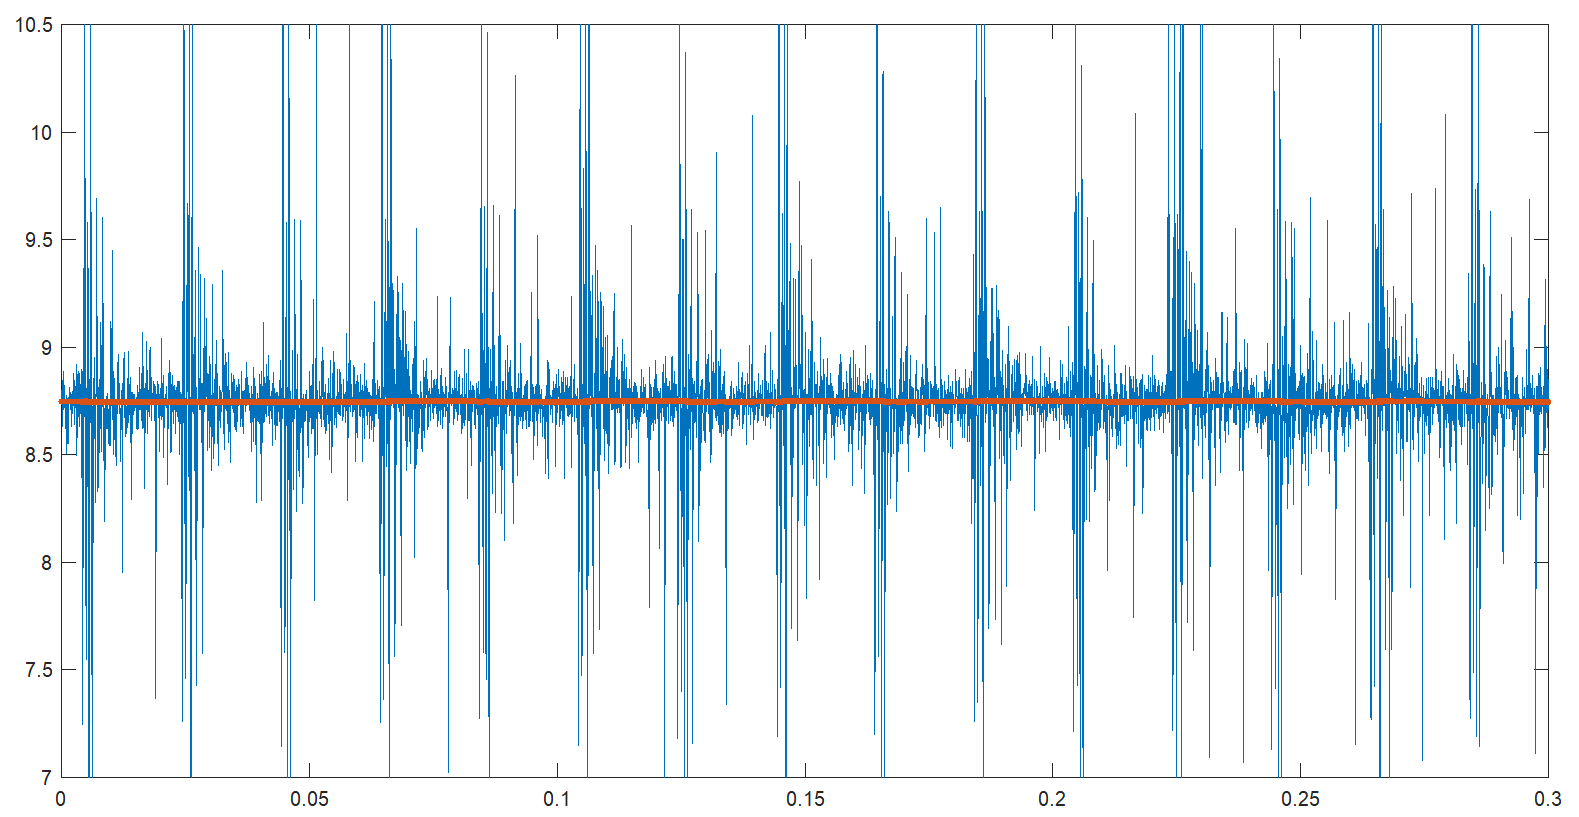
\includegraphics[width=\textwidth]{../Pictures/P1/Discussion/sw_filter_current.png}
		\caption{Current measurement against time. Both software filtered (red) and raw (blue) signals can be seen. The filtered signal data points' size has been increased to improve readability.}
		\label{software_filter}
	\end{center}	
\end{figure}


\subsection{Inductor}
\label{Coil problems}
Since the scope of the project was the validation of the converter, it was decided to implement an existing inductor. A coil was then selected with an approximate inductance of slightly over $1mH$.
The PCB was then designed for this initial inductor. However, after some  tests under high currents it was shown that the coil was not maintaining its inductance due to saturation of the core. Also, it was reaching temperatures over $100\dec C$. The inductance was then tested under different currents and the behavior was verified as shown in figure \ref{Coil comparison}.

It was then decided to implement another inductor which would satisfy the requirements in all cases. The same tests were performed for the new inductor and it was shown that it would fulfill the requirements without problems. 
Also, some thermal tests were performed on the new inductor. With a constant current of $10A$, it shows a maximum temperature of $60\dec C$ after 10 minutes.

\begin{figure}[H]
	\begin{center}
		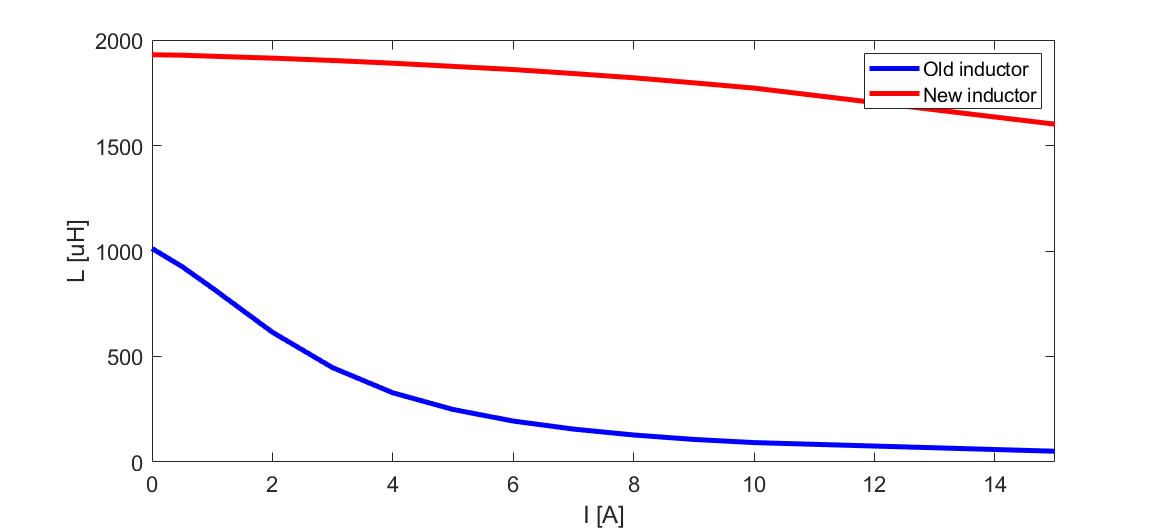
\includegraphics[width=1\textwidth]{docs/discussion/CoilTests/CoilComparison50kHzV2.png}
		\caption{Inductor comparison under changes on current flow (50kHz).}
		\label{Coil comparison}
	\end{center}	
\end{figure}

However, the size and weight of the new inductor are much higher than those of the previous one. This means that the footprint designed is not valid for the new coil and it hangs loose outside the PCB.



\section{Future work}
This section will describe the planned future work of the project. This includes parts that were prioritized low or Simplified to achieve a working converter. Furthermore it includes improvements that was discovered during both the development and testing period of the project.

%4- Recommendations for future work. Make general statements. Items: a)what study is needed, b)Methods to be used, c)what is needed for that study.

\subsection{MPPT technique}
Even though the P\&O algorithm was implemented, initial research showed that the incremental conductance method could have been a better option.  Further research and simulations will have to be made for comparing the two methods. \todo{Write about what could be gained from changing MPPT, NHF.}

\subsection{V/I controller}


\subsection{Hardware improvements}
In the first iterations of the converter design, the driver circuits have been designed using isolated power supplies for the high side drivers. These are costly both in size and money wise. Because of that it's preferable to implement a bootstrap circuit for the drivers. An option for a driver including bootstrap could be UCC27211 \cite{boot_driver_datasheet}. This includes both a high and low side driver, such that only to IC's are necessary for the converter. The input threshold is below $2.8V$ for both sides, which means that a $5V$ optocoupler could be used for isolation. For cost and size optimization the optocouplers should be one quad optocoupler, instead of four singles. 
 
%bootstrap, change driver to the A version due to voltage levels and then change the optocouupler to a quad version, control system powered from pv-panel, \dots

\subsection{Coil design}
The coil used for the converter is reused from an earlier project. Measurements shows that it's oversized regarding current ratings. To achieve an optimal coil it should be designed for this specific converter. Both the core size and wire diameter depends on the wanted current rating of the converter \cite{underthehood}. Because of this it will be possible to lower both the cost and size of the coil. 

\subsection{Switching frequency limitations}

%\subsection{Component price, system size, optimization needed}
%Component prize and system size will be introduced during the other sections...

\subsection{Efficiency}
The main purpose of the MIC is to maximize the output efficiency of a PV-panel. To achieve that, the efficiency of the converter itself should be maximized. During the tests, the efficiency was measured to \textit{ADD SOME NICE DATA}\todo{Insert measured efficiency, NHF.}. Other papers shows that an efficiency of up to $95-96\%$ should be achievable\cite{underthehood}, \cite{efficient_buckboost}. 




